\documentclass[conference]{IEEEtran}
\usepackage[utf8]{inputenc}
\usepackage[T1]{fontenc}
\usepackage[polish]{babel}
\usepackage{graphicx}
\usepackage{amsmath}
\usepackage{cite}
\usepackage{url}

\begin{document}

% ====================================================================
% TYTUŁ, AUTOR i NUMERACJA STRON
% ====================================================================
    
    \title{Porównanie efektywności algorytmów dokładnych i heurystycznych dla Problemu Komiwojażera (TSP)}
    \author{
        \IEEEauthorblockN{Kacper Piekut}
        \IEEEauthorblockA{Numer albumu: 280879\\
        Wydział: W4N, Rok akademicki: 2025/2026, Semestr: 6\\
        Politechnika Wrocławska}
        }
    \maketitle
    \thispagestyle{empty}
    \pagestyle{plain}

% ====================================================================
% ABSTRAKT
% ====================================================================

    \begin{abstract}
        W niniejszym sprawozdaniu przedstawiono analizę i porównanie czterech algorytmów rozwiązujących Problem Komiwojażera w wariancie symetrycznym (STSP) oraz asymetrycznym (ATSP): Przeglądu Zupełnego (Brute-Force), błądzenia losowego (RAND), Najbliższego Sąsiada (NN) oraz powtarzalnego Najbliższego Sąsiada (RNN). Badania przeprowadzono na wygenerowanych instancjach losowych oraz na grafach z biblioteki TSPLIB, w tym na specyficznych instancjach technologicznych (VLSI/PCB). Wyniki potwierdzają wykładniczą złożoność algorytmu Brute-Force oraz ukazują charakterystykę zbieżności algorytmu losowego. Wykazano również drastyczny kompromis pomiędzy czasem obliczeń a gwarancją optymalności.
    \end{abstract}
    \begin{IEEEkeywords}
        Problem Komiwojażera, Algorytmy Heurystyczne, Złożoność Obliczeniowa, Cykl Hamiltona, TSPLIB, VLSI, TSP, ATSP.
    \end{IEEEkeywords}

% ====================================================================
% I. WSTĘP I HIPOTEZY
% ====================================================================

    \section{Wstęp}
        \subsection{Hipotezy badawcze}
            Przed przystąpieniem do pomiarów sformułowano następujące hipotezy, odpowiadające na pytania badawcze:
            \begin{itemize}
                \item \textbf{H1 (Złożoność Brute-Force):} Czas obliczeń algorytmu dokładnego rośnie w tempie silni ($O((N-1)!)$), co sprawi, że przekroczy on założony limit 30 minut już dla instancji $N \ge 15$, niezależnie od tego, czy graf jest symetryczny, czy asymetryczny.
                \item \textbf{H2 (Kompromis i wyznaczanie UB):} Istnieje drastyczny kompromis między czasem a jakością. Metody heurystyczne wyznaczą rozwiązania o kilka rzędów wielkości szybciej niż metoda dokładna, co czyni je bardzo efektywnymi metodami do błyskawicznego wyznaczania górnego ograniczenia (UB) dla algorytmów dokładnych.
                \item \textbf{H3 (Zbieżność RAND i warunek stopu):} Prawdopodobieństwo znalezienia lepszej trasy przez algorytm losowy maleje z upływem czasu, prowadząc do stagnacji. Pozwala to na zastąpienie sztywnego limitu czasowego warunkiem braku poprawy, drastycznie skracając czas badań bez utraty wiarygodności wyników.
                \item \textbf{H4 (Wpływ wierzchołka startowego):} Wynik klasycznego algorytmu zachłannego (NN) jest krytycznie uzależniony od wyboru początkowego miasta. Iteracyjne sprawdzenie każdego punktu startowego (RNN) zagwarantuje znalezienie trasy o koszcie mniejszym lub równym.
            \end{itemize}

% ====================================================================
% II. METODOLOGIA BADAŃ
% ====================================================================

    \section{Metodologia Badań}
        \subsection{Środowisko testowe i dane wejściowe}
            Badania przeprowadzono na laptopie ASUS TUF Gaming F15 (procesor Intel Core i5-11400H 2.7-4.5 GHz, 16 GB RAM DDR4, dysk SSD NVMe 512 GB) pod kontrolą systemu Windows 11 Home (64-bit). Środowiskiem programistycznym był język C++ (kompilator MinGW GCC). 
            W badaniach wykorzystano dwa źródła danych:
            \begin{itemize}
                \item \textbf{Generowane losowo grafy pełne:} wygenerowano zestawy instancji symetrycznych i asymetrycznych o rozmiarach $N \in \langle 6, 15 \rangle$ dla algorytmu Brute-Force oraz $N=11$ do weryfikacji kompromisu czasowego. Krawędzie losowano z rozkładu jednostajnego z przedziału $\langle 1, 100 \rangle$.
                \item \textbf{Biblioteka TSPLIB:} wykorzystano klasyczne instancje geograficzne oraz specjalistyczne instancje technologiczne VLSI.
            \end{itemize}
        \subsection{Opis zaimplementowanych algorytmów}
            % JAK STARCZY CZAS:
            % \begin{figure}[htbp]
            %     \centerline{\includegraphics[width=\columnwidth]{schemat_rnn.png}}
            %     \caption{Schemat blokowy działania algorytmu RNN z uwzględnieniem nawrotów (DFS) dla krawędzi o identycznych wagach.}
            %     \label{fig:schemat_rnn}
            % \end{figure}
            Badaniom poddano cztery implementacje algorytmów rozwiązujących Problem Komiwojażera:
            \begin{itemize}
                \item \textbf{Błądzenie Losowe (RAND):} Metoda losująca permutacje w pętli aż do momentu osiągnięcia limitu czasu lub odnalezienia rozwiązania optymalnego. Zastosowano mechanizm blokowania pierwszego miasta w celu zminimalizowania ryzyka powtórnego wylosowania tego samego cyklu Hamiltona.
                \item \textbf{Najbliższy Sąsiad (NN):} Metoda zachłanna, która zaczynając od zadanego wierzchołka, w każdym kroku dobiera najbliższe, nieodwiedzone jeszcze miasto.
                \item \textbf{Powtarzalny Najbliższy Sąsiad (RNN):} Rozszerzenie algorytmu NN. Metoda iteruje po każdym z $N$ wierzchołków grafu traktując go jako potencjalny start. Dodatkowo, implementacja uwzględnia obsługę remisów (równych wag) poprzez tworzenie rozgałęzień i sprawdzanie wszystkich możliwych dróg o tym samym lokalnym koszcie minimalnym.
                \item \textbf{Przegląd Zupełny (Brute-Force):} Metoda dokładna generująca wszystkie możliwe permutacje wierzchołków. W celu optymalizacji przestrzeni poszukiwań również zastosowano blokowanie pierwszego wierzchołka (jak w metodzie RAND), redukując liczbę permutacji z $N!$ do $(N-1)!$.
            \end{itemize}
        \subsection{Konfiguracja eksperymentu}
            Aplikacja testowa została zaprojektowana w sposób wykluczający twarde kodowanie. Całym przepływem steruje zewnętrzny plik tekstowy \texttt{config.txt}. Przykładowa konfiguracja uruchamiająca badanie algorytmu RNN z limitem 15 minut (900 sekund) i 100 powtórzeniami prezentuje się następująco:
\begin{verbatim}
 ALGORITHM = RNN
 GRAPH_PATH = data/tsplib/tsp/berlin52.tsp
 GENERATE_NEW = false
 OPTIMAL_COST = 7542
 TIME_LIMIT_SECONDS = 900
 REPETITIONS = 100
 SAVE_TO_CSV = true
\end{verbatim}
        \subsection{Procedura badawcza i miary oceny}
            Eksperymenty podzielono na dwie fazy. W pierwszej fazie weryfikowano algorytmy dokładne, mierząc całkowity czas znalezienia globalnego optimum w zależności od rozmiaru $N$ oraz typu symetrii grafu. W drugiej fazie weryfikowano metody heurystyczne. 
            Jakość rozwiązań heurystycznych oceniano za pomocą błędu względnego $\delta$, który wyraża procentowy wzrost kosztu znalezionej trasy względem optymalnego, znanego rozwiązania:
            \begin{equation}
                \delta = \frac{Koszt_{alg} - Koszt_{opt}}{Koszt_{opt}} \cdot 100\%
            \end{equation}
            Aby zniwelować wpływ procesów systemowych na precyzję pomiarów czasu, procedura badawcza zakładała wielokrotne uruchamianie algorytmu dla danej instancji (zgodnie z parametrem \texttt{REPETITIONS}). Program dokonywał agregacji wyników, obliczając średni czas wykonania, podczas gdy koszt końcowy stanowił najlepszy (minimalny) wynik uzyskany ze wszystkich powtórzeń.
        \subsection{Teoretyczna złożoność i przestrzeń poszukiwań}
            Dla algorytmu dokładnego (Brute-Force) oraz algorytmu losowego (RAND) wspólną przestrzenią poszukiwań jest zbiór wszystkich cykli Hamiltona. Dzięki optymalizacji zablokowania startu, rozmiar przestrzeni $P$ wynosi:
            \begin{equation}
                P = (N - 1)!
            \end{equation}
            Z kolei dla algorytmów zachłannych zdefiniowano teoretyczną złożoność obliczeniową. Algorytm Najbliższego Sąsiada (NN) w każdym z $N$ kroków przeszukuje listę malejącej liczby nieodwiedzonych sąsiadów, co daje złożoność rzędu $O(N^2)$. Algorytm powtarzalny (RNN), sprawdzając dodatkowo wszystkie starty, zwiększa tę złożoność do $O(N^3)$.
        \subsection{Metodyka szacowania maksymalnego rozmiaru instancji}
            Zakładając, że czas wykonania algorytmu $t$ jest proporcjonalny do jego teoretycznej złożoności $f(N)$, można wprowadzić sprzętową stałą proporcjonalności $c$:
            \begin{equation}
                t \approx c \cdot f(N)
            \end{equation}
            Znając czas wykonania $t$ dla konkretnego, zbadanego rozmiaru instancji $N$, stałą $c$ dla danego środowiska obliczeniowego wyznacza się ze wzoru:
            \begin{equation}
                c = \frac{t}{f(N)}
            \end{equation}
            Posiadając wyznaczoną stałą proporcjonalności, można przekształcić równanie, aby oszacować maksymalny rozmiar instancji $N_{max}$, który system jest w stanie przetworzyć w limicie czasowym $T_{limit}$. Dla algorytmów o złożoności kwadratowej $\mathcal{O}(N^2)$ oraz sześciennej $\mathcal{O}(N^3)$, wzory przyjmują odpowiednio postać:
            \begin{equation}
                N_{max} = \sqrt{\frac{T_{limit}}{c}}
            \end{equation}
            \begin{equation}
                N_{max} = \sqrt[3]{\frac{T_{limit}}{c}}
            \end{equation}

% ====================================================================
% III. WYNIKI BADAŃ
% ====================================================================

    \section{Wyniki Badań}
        \subsection{Złożoność algorytmu Brute-Force (Sym. vs Asym.)}
            Wygenerowano dwa zbiory grafów pełnych o rozmiarach od $N=6$ do $N=15$. Zestawienie czasów wykonania algorytmu Brute-Force przedstawia Tabela \ref{tab:bruteforce} oraz wykresy \ref{fig:time_vs_size_sym} i \ref{fig:time_vs_size_asym}.
            \begin{table}[htbp]
                \caption{Porównanie czasu wykonania algorytmu Brute-Force dla grafów symetrycznych i asymetrycznych}
                \begin{center}
                \begin{tabular}{|c|c|c|c|}
                \hline
                \textbf{N} & \textbf{P} & \textbf{Czas - Sym. [us]} & \textbf{Czas - Asym. [us]} \\ \hline
                6 & 120 & $9{,}60 \cdot 10^{0}$ & $1{,}24 \cdot 10^{1}$ \\ \hline
                7 & 720 & $4{,}26 \cdot 10^{1}$ & $3{,}96 \cdot 10^{1}$ \\ \hline
                8 & 5\,040 & $2{,}86 \cdot 10^{2}$ & $2{,}64 \cdot 10^{2}$ \\ \hline
                9 & 40\,320 & $2{,}17 \cdot 10^{3}$ & $2{,}14 \cdot 10^{3}$ \\ \hline
                10 & 362\,880 & $1{,}99 \cdot 10^{4}$ & $1{,}96 \cdot 10^{4}$ \\ \hline
                11 & 3\,628\,800 & $1{,}85 \cdot 10^{5}$ & $1{,}87 \cdot 10^{5}$ \\ \hline
                12 & 39\,916\,800 & $2{,}11 \cdot 10^{6}$ & $2{,}12 \cdot 10^{6}$ \\ \hline
                13 & 479\,001\,600 & $2{,}52 \cdot 10^{7}$ & $2{,}53 \cdot 10^{7}$ \\ \hline
                14 & 6\,227\,020\,800 & $3{,}43 \cdot 10^{8}$ & $3{,}39 \cdot 10^{8}$ \\ \hline
                15 & 87\,178\,291\,200 & TimeOut & TimeOut \\ \hline
                \end{tabular}
                \label{tab:bruteforce}
                \end{center}
            \end{table}
            \begin{figure}[htbp]
                \centerline{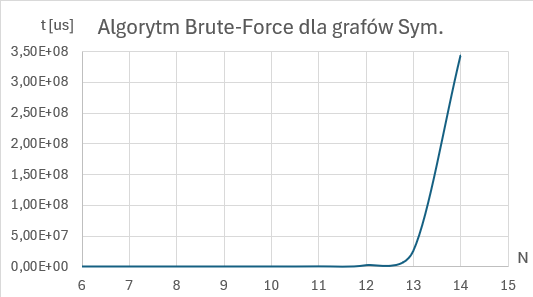
\includegraphics[width=\columnwidth]{images/wykres_brute_force_sym.png}}
                \caption{Zależność czasu wykonywania od rozmiaru instancji ($N$) dla algorytmu Brute-Force (grafy symetryczne).}
                \label{fig:time_vs_size_sym}
            \end{figure}
            \begin{figure}[htbp]
                \centerline{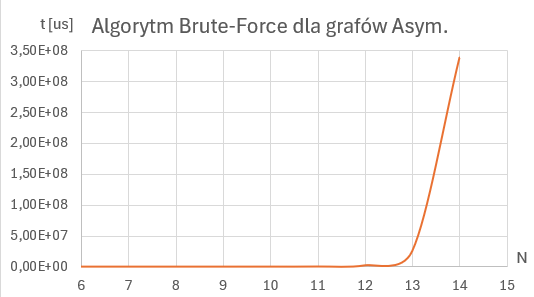
\includegraphics[width=\columnwidth]{images/wykres_brute_force_asym.png}}
                \caption{Zależność czasu wykonywania od rozmiaru instancji ($N$) dla algorytmu Brute-Force (grafy asymetryczne).}
                \label{fig:time_vs_size_asym}
            \end{figure}
        \subsection{Złożoność i ograniczenia czasowe algorytmu RAND}
            Przeprowadzono badanie algorytmu błądzenia losowego (RAND) na wygenerowanych instancjach o rozmiarach od $N=6$ do $N=13$ (Tabela \ref{tab:rand_czas}, wykres \ref{fig:rand_time_vs_size}). Ponieważ założony limit czasowy (30 minut) był wystarczający na odnalezienie optimum, błąd względny dla wszystkich poniższych pomiarów wyniósł 0\%. W związku z tym w poniższym zestawieniu pominięto kolumnę błędu, skupiając się wyłącznie na drastycznym wzroście czasu wykonania algorytmu.\\
            \begin{table}[htbp]
                \caption{Czas poszukiwania rozwiązania optymalnego przez algorytm RAND}
                \begin{center}
                \begin{tabular}{|c|c|c|c|}
                \hline
                \textbf{N} & \textbf{P} & \textbf{Czas - Sym. [us]} & \textbf{Czas - Asym. [us]} \\ \hline
                6 & 120 & $7{,}60 \cdot 10^{0}$ & $2{,}10 \cdot 10^{1}$ \\ \hline
                7 & 720 & $4{,}96 \cdot 10^{1}$ & $2{,}80 \cdot 10^{1}$ \\ \hline
                8 & 5\,040 & $1{,}62 \cdot 10^{2}$ & $2{,}28 \cdot 10^{2}$ \\ \hline
                9 & 40\,320 & $5{,}94 \cdot 10^{2}$ & $3{,}82 \cdot 10^{3}$ \\ \hline
                10 & 362\,880 & $1{,}96 \cdot 10^{4}$ & $4{,}72 \cdot 10^{4}$ \\ \hline
                11 & 3\,628\,800 & $1{,}32 \cdot 10^{5}$ & $3{,}51 \cdot 10^{5}$ \\ \hline
                12 & 39\,916\,800 & $1{,}95 \cdot 10^{6}$ & $4{,}38 \cdot 10^{6}$ \\ \hline
                13 & 479\,001\,600 & $9{,}32 \cdot 10^{6}$ & $4{,}60 \cdot 10^{7}$ \\ \hline
                \end{tabular}
                \label{tab:rand_czas}
                \end{center}
            \end{table}
            \begin{figure}[htbp]
                \centerline{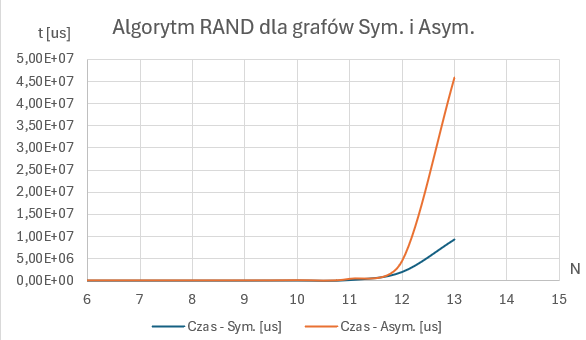
\includegraphics[width=\columnwidth]{images/wykres_RAND_czas.png}}
                \caption{Zależność czasu wykonywania od rozmiaru instancji ($N$) dla algorytmu RAND.}
                \label{fig:rand_time_vs_size}
            \end{figure}
            Następnie, oszacowano maksymalny rozmiar instancji $N$, dla której algorytm losowy jest w stanie znaleźć optimum w rozsądnym czasie 30 minut. Należy zaznaczyć, że przestrzeń poszukiwań algorytmu RAND to zawsze zbiór wszystkich cykli Hamiltona wynoszący $P = (N-1)!$, niezależnie od tego, czy instancja jest generowana losowo, pochodzi z TSPLIB czy jest siatką VLSI (algorytm losuje trasy w ciemno, ignorując wagi krawędzi). Z tego powodu oszacowanie maksymalnego $N$ opiera się wyłącznie na uniwersalnej przepustowości obliczeniowej zaimplementowanego algorytmu.
            W celu weryfikacji przepustowości uruchomiono algorytm na instancji \texttt{berlin52.tsp} z rygorystycznym limitem 1 minuty. W tym czasie program wygenerował i ocenił dokładnie $304\,686\,769$ tras. Dokonując liniowej ekstrapolacji, w czasie 30 minut algorytm jest w stanie sprawdzić $C_{max}$ unikalnych tras:
            \begin{equation}
                C_{max} = 30 \cdot 304\,686\,769 \approx 9{,}14 \cdot 10^9 \text{ tras}
            \end{equation}
        \subsection{Historia zbieżności algorytmu RAND}
            W celu szczegółowego zbadania charakterystyki pracy algorytmu losowego, zarejestrowano proces poprawy najlepszego znalezionego rozwiązania w trakcie trwania obliczeń. Analizę przeprowadzono na podstawie pliku z historią wykonania (\texttt{history\_RAND.csv}) dla instancji o rozmiarze $N=13$. Zarejestrowane punkty pomiarowe, obrazujące zmianę kosztu najkrótszej odnalezionej trasy w funkcji upływającego czasu, naniesiono na wykres przedstawiony na Rysunku \ref{fig:rand_historia}.
            \begin{figure}[htbp]
                \centerline{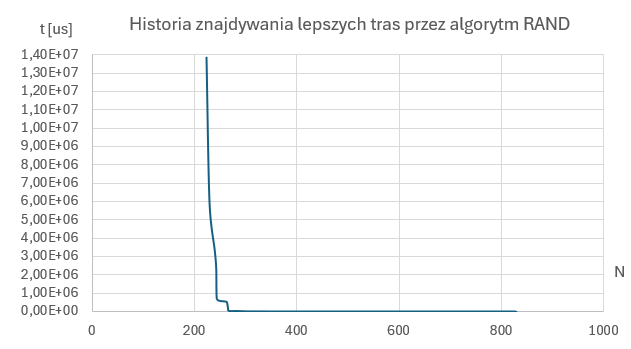
\includegraphics[width=\columnwidth]{images/wykres_rand_historia.png}}
                \caption{Krzywa zbieżności algorytmu RAND dla instancji o rozmiarze $N=13$. Wykres przedstawia zmianę kosztu najlepszej znalezionej trasy w funkcji czasu wyrażonego w mikrosekundach.}
                \label{fig:rand_historia}
            \end{figure}
        \vspace{3mm}
        \subsection{Efektywność i błąd względny algorytmów NN i RNN}
            Przeprowadzona została analiza metod: algorytmu Najbliższego Sąsiada (NN) oraz jego rozszerzonej wersji, sprawdzającej każdy możliwy wierzchołek startowy (RNN). 
            W pierwszej kolejności zestawiono czasy wykonania tych metod z algorytmem losowym (RAND). Zależność tę, w skali logarytmicznej, przedstawiono na Rysunku \ref{fig:rand_nn_rnn_czas}.
            Wyniki dla wygenerowanych instancji symetrycznych i asymetrycznych zestawiono w Tabeli \ref{tab:nn_rnn_blad} oraz zobrazowano na Rysunku \ref{fig:nn_rnn_blad}.
            \begin{figure}[htbp]
                \centerline{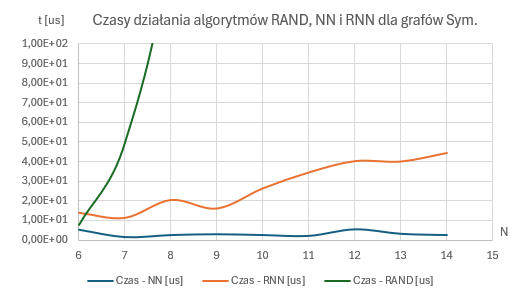
\includegraphics[width=\columnwidth]{images/wykres_RAND_NN_RNN_czas.png}}
                \caption{Porównanie czasu wykonania algorytmów RAND, NN i RNN w zależności od rozmiaru instancji ($N$). Oś Y w skali logarytmicznej.}
                \label{fig:rand_nn_rnn_czas}
            \end{figure}
            \begin{table}[htbp]
                \caption{Porównanie błędu względnego algorytmów NN i RNN}
                \begin{center}
                \begin{tabular}{|c|c|c|c|}
                \hline
                \textbf{N} & \textbf{Instancja} & \textbf{$\delta$ NN [\%]} & \textbf{$\delta$ RNN [\%]} \\ \hline
                6 & sym\_6 & $28{,}47\%$ & $0{,}00\%$ \\ \hline
                7 & sym\_7 & $22{,}63\%$ & $22{,}63\%$ \\ \hline
                8 & sym\_8 & $15{,}81\%$ & $0{,}00\%$ \\ \hline
                9 & sym\_9 & $0{,}00\%$ & $0{,}00\%$ \\ \hline
                10 & sym\_10 & $47{,}85\%$ & $13{,}40\%$ \\ \hline
                11 & sym\_11 & $43{,}48\%$ & $0{,}00\%$ \\ \hline
                12 & sym\_12 & $67{,}10\%$ & $0{,}00\%$ \\ \hline
                14 & sym\_14 & $4{,}44\%$ & $4{,}44\%$ \\ \hline
                6 & asym\_6 & $0{,}00\%$ & $0{,}00\%$ \\ \hline
                7 & asym\_7 & $29{,}73\%$ & $0{,}54\%$ \\ \hline
                8 & asym\_8 & $59{,}12\%$ & $2{,}19\%$ \\ \hline
                9 & asym\_9 & $56{,}35\%$ & $0{,}00\%$ \\ \hline
                10 & asym\_10 & $66{,}03\%$ & $3{,}21\%$ \\ \hline
                11 & asym\_11 & $62{,}31\%$ & $6{,}92\%$ \\ \hline
                12 & asym\_12 & $89{,}08\%$ & $38{,}66\%$ \\ \hline
                14 & asym\_14 & $40{,}98\%$ & $39{,}51\%$ \\ \hline
                \end{tabular}
                \label{tab:nn_rnn_blad}
                \end{center}
            \end{table}
            \begin{figure}[htbp]
                \centerline{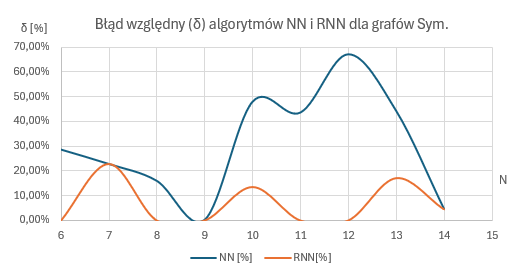
\includegraphics[width=\columnwidth]{images/wykres_NN_RNN_blad_wzgledny.png}}
                \caption{Wykres słupkowy prezentujący zestawienie błędu względnego dla algorytmów NN i RNN na badanych instancjach.}
                \label{fig:nn_rnn_blad}
            \end{figure}
        \subsection{Maksymalny rozmiar instancji dla algorytmów NN i RNN dla limitu czasowego}
            Podjęta została próba oszacowania maksymalnego rozmiaru grafu ($N$), dla którego algorytmy zachłanne znajdą rozwiązanie w czasie 15 minut ($9 \cdot 10^8 \text{ }\mu\text{s}$). Ponieważ zbadane metody charakteryzują się złożonością wielomianową, wyliczeń dokonano na podstawie stałej proporcjonalności $c$ wyznaczonej dla instancji $N=14$.
            Dla algorytmu Najbliższego Sąsiada (NN) o złożoności $\mathcal{O}(N^2)$ czas wykonania dla $N=14$ wyniósł $t = 2{,}6 \text{ }\mu\text{s}$.
            \begin{equation}
                c_{NN} = \frac{t}{N^2} = \frac{2{,}6}{14^2} \approx 0{,}0132 \text{ }\mu\text{s}
            \end{equation}
            Przyrównując to do limitu 15 minut, otrzymujemy maksymalny rozmiar problemu:
            \begin{equation}
                N_{max\_NN} = \sqrt{\frac{9 \cdot 10^8}{0{,}0132}} \approx 261\,000 \text{ wierzchołków}
            \end{equation}
            Dla algorytmu powtarzalnego (RNN) o złożoności $\mathcal{O}(N^3)$ czas dla $N=14$ wyniósł $t = 44{,}6 \text{ }\mu\text{s}$.
            \begin{equation}
                c_{RNN} = \frac{t}{N^3} = \frac{44{,}6}{14^3} \approx 0{,}0162 \text{ }\mu\text{s}
            \end{equation}
            \begin{equation}
                N_{max\_RNN} = \sqrt[3]{\frac{9 \cdot 10^8}{0{,}0162}} \approx 3\,800 \text{ wierzchołków}
            \end{equation}
        \subsection{Weryfikacja błędu względnego na instancjach TSPLIB i VLSI}
            Została przeprowadzona konfrontacja zaimplementowanych algorytmów z rzeczywistymi, ustandaryzowanymi instancjami problemu z biblioteki TSPLIB (\texttt{berlin52.tsp}, \texttt{ft53.atsp}) oraz siatką punktów VLSI (\texttt{pia3056.tsp}). Algorytmy zachłanne (NN i RNN) z racji swojej wielomianowej złożoności rozwiązały te instancje błyskawicznie. Algorytmowi losowemu (RAND) narzucono w tym teście rygorystyczny limit czasowy wynoszący 1 minutę, badając jakość rozwiązania, jakie jest w stanie wygenerować w krótkim oknie czasowym.
            \begin{table}[htbp]
                \caption{Błąd względny algorytmów dla instancji TSPLIB i VLSI}
                \begin{center}
                \begin{tabular}{|c|c|c|c|c|c|}
                \hline
                \textbf{Instancja} & \textbf{Typ} & \textbf{N} & \textbf{$\delta$ NN} & \textbf{$\delta$ RNN} & \textbf{$\delta$ RAND (60s)} \\ \hline
                berlin52 & STSP & 52 & $19{,}07\%$ & $8{,}47\%$ & $161{,}75\%$ \\ \hline
                ft53 & ATSP & 53 & $25{,}75\%$ & $9{,}63\%$ & $434{,}63\%$ \\ \hline
                pia3056 & VLSI & 3056 & $22{,}03\%$ & $16{,}82\%$ & $2186{,}41\%$ \\ \hline
                \end{tabular}
                \label{tab:tsplib_vlsi_blad}
                \end{center}
            \end{table}

% ====================================================================
% IV. DYSKUSJA I WNIOSKI
% ====================================================================

    \section{Dyskusja i Wnioski}
        \subsection{Weryfikacja hipotez badawczych}
            Na podstawie przeprowadzonych eksperymentów i zebranych danych analitycznych, zweryfikowano hipotezy postawione we wstępie:
            \begin{itemize}
                \item \textbf{H1 (Złożoność Brute-Force) - Potwierdzona.} Pomiary czasu wykazały wzrost zgodny z krzywą silni. Dla instancji $N=15$ algorytm nie odnalazł rozwiązania w racjonalnym czasie i przekroczył narzucony limit, niezależnie od tego, czy badany graf był symetryczny, czy asymetryczny.
                \item \textbf{H2 (Kompromis i wyznaczanie UB) - Potwierdzona.} Zaobserwowano przepaść wydajnościową. Algorytmy heurystyczne rozwiązują problemy wielokrotnie szybciej, dostarczając bardzo dobre wyniki startowe. Czyni to z nich perfekcyjne narzędzie do błyskawicznego wyznaczania Górnego Ograniczenia (UB).
                \item \textbf{H3 (Zbieżność RAND i warunek stopu) - Potwierdzona.} Analiza krzywej zbieżności uwidoczniła szybkie wejście algorytmu losowego w stan długotrwałej stagnacji. Zastąpienie limitu czasowego warunkiem ucinania algorytmu po z góry ustalonej liczbie pustych iteracji pozwala drastycznie zredukować czas poszukiwań przy zachowaniu identycznej jakości.                
                \item \textbf{H4 (Wpływ wierzchołka startowego) - Potwierdzona.} Narzucenie pojedynczego miasta startowego w algorytmie NN prowadziło w wielu przypadkach do suboptymalnych decyzji. Zastosowanie iteracji po wszystkich wierzchołkach (RNN) całkowicie zniwelowało to ryzyko, co przełożyło się na bezwzględną poprawę precyzji.
            \end{itemize}
        \subsection{Złożoność obliczeniowa i skalowalność}
            Wyznaczona została złożoność obliczeniową badanych metod. Czasy wykonania algorytmu Brute-Force odwzorowują krzywą silni, potwierdzając jego teoretyczną złożoność $\mathcal{O}((N-1)!)$. Dodatkowo, brak widocznych różnic w czasie dla grafów symetrycznych i asymetrycznych dowodzi, że czas działania algorytmu jest całkowicie niezależny od topologii i wagi krawędzi.
            W drastycznym kontraście pozostają algorytmy zachłanne. Dla reprezentacji macierzowej, algorytm Najbliższego Sąsiada (NN) w każdym z $N$ kroków przeszukuje listę malejącej liczby nieodwiedzonych wierzchołków. Stanowi to sumę ciągu arytmetycznego, dając złożoność wielomianową $\mathcal{O}(N^2)$. Z kolei wersja powtarzalna (RNN), jako rozszerzenie polegające na iteracji przez wszystkie $N$ możliwych miast startowych, powiększa ten czas $N$-krotnie, podnosząc złożoność do $\mathcal{O}(N^3)$. Jak wykazały badania (Rys. \ref{fig:rand_nn_rnn_czas}), oba te rzędy wielkości dla grafów z rzędu $N \le 15$ dają czasy egzekucji liczone w ułamkach milisekund, gwarantując potężną skalowalność niedostępną algorytmom dokładnym.
            Narzucanie limitów czasowych (np. 30 minut) jest koniecznością dla algorytmów klasy Brute-Force oraz RAND z uwagi na fizyczną i technologiczną niemożliwość przeszukania przestrzeni rosnącej w tempie silni. Z kolei dla algorytmów wielomianowych (NN i RNN) limit 15 minut jest przydatny - pozwala on na przetwarzanie gigantycznych grafów, przez co w praktyce dla mniejszych instancji limit ten nie ma żadnego znaczenia i nigdy nie zostaje osiągnięty.
        \subsection{Zjawisko stagnacji i ograniczenie czasu w algorytmie RAND}
            Na podstawie matematycznych obliczeń przepustowości wykazano, że 30-minutowe ramy czasowe są niewystarczające, aby algorytm RAND mógł odnaleźć optimum dla grafów z biblioteki TSPLIB.
            Przeanalizowano również możliwość zastąpienia sztywnego, 30-minutowego limitu innym, bardziej racjonalnym kryterium stopu. Analiza wygenerowanej krzywej zbieżności (Rys. \ref{fig:rand_historia}) daje jednoznaczną odpowiedź: \textbf{czas działania algorytmu probabilistycznego można znacząco skrócić poprzez zastosowanie warunku braku poprawy rozwiązania (stagnacji)}.
            Wykres udowadnia, że metoda losowa początkowo błyskawicznie znajduje akceptowalne trasy, po czym wpada w bardzo długie, płaskie fazy bezczynności. Znacznie efektywniejszym i wiarygodnym kryterium stopu jest odliczanie pustych iteracji - jeżeli przez ustalony próg (np. 1 milion wylosowanych tras) algorytm nie znajdzie lepszego kosztu, dalsze obliczenia powinny zostać przerwane.
            Aby zapewnić brak powtarzających się permutacji przy zachowaniu w pełni losowego charakteru, jedną z najskuteczniejszych metod jest zastosowanie generatora liczb pseudolosowych (Mersenne Twister \texttt{std::mt19937} ze standardu C++ w połączeniu ze \texttt{std::shuffle}), co gwarantuje równomierny rozkład prawdopodobieństwa tasowania wierzchołków.
        \subsection{Efektywność heurystyk i wyznaczanie ograniczeń (UB)}
            Odpowiadając na jedno z kluczowych pytań projektu: \textbf{kiedy i dlaczego rozwiązanie RNN jest korzystniejsze niż NN?} 
            Badania (Tab. \ref{tab:nn_rnn_blad}) udowodniły, że klasyczny algorytm NN, ze względu na swój skrajny optymizm lokalny, podejmuje gorsze decyzje. Rozwiązanie RNN jest bezwzględnie korzystniejsze w każdej sytuacji, w której nie jesteśmy rygorystycznie ograniczeni czasem. Poświęcając minimalnie więcej mocy obliczeniowej (z $\mathcal{O}(N^2)$ na $\mathcal{O}(N^3)$), omijamy ryzyko wyboru najgorszego wierzchołka startowego, z którego nie ma dobrego wyjścia do reszty grafu, często niwelując błąd względny do $0\%$ na małych instancjach.
            \textbf{Górne i Dolne Ograniczenie (UB i LB):}
            W kontekście rozwiązywania TSP, Górne Ograniczenie (UB) to koszt najgorszego akceptowalnego rozwiązania, stanowiący próg odcinania gorszych tras. Dolne Ograniczenie (LB) to z kolei teoretyczny koszt idealnej trasy. 
            Jak wykazały pomiary, algorytmy NN i RNN są perfekcyjnymi, superszybkimi generatorami bardzo silnego (niskiego) UB. W ułamek sekundy dostarczają trasę o dobrej jakości. Z kolei używanie do tego celu algorytmu RAND jest nieefektywne z powdu osiągania gorszych wyników czasowych i jakościowych.
        \subsection{Wpływ parametrów instancji na złożoność zbadanych algorytmów}
            Odpowiadając na pytania badawcze, przeanalizowano wpływ struktury grafu na działanie algorytmów:
            \begin{itemize}
                \item \textbf{Gęstość grafu:} Zbadane tu algorytmy (Brute-Force, RAND, NN, RNN) w swojej naiwnej postaci zakładają pełną macierz sąsiedztwa i nie korzystają z odcinania. W związku z tym brak krawędzi (mniejsza gęstość) nie zmniejsza liczby iteracji - program nadal musi sprawdzić $O((N-1)!)$ lub wykonać $N^k$ kroków.\\
                \item \textbf{Wiele ścieżek o optymalnym koszcie:} Fakt ten nie ma absolutnie żadnego wpływu na algorytmy Brute-Force, NN czy RNN, które działają deterministycznie lub muszą sprawdzić całą przestrzeń. Ma jednak pozytywny wpływ na algorytm RAND - zagęszczenie optymalnych rozwiązań w przestrzeni drastycznie zwiększa prawdopodobieństwo trafienia optimum w krótszym czasie.
                \item \textbf{Zakres wag krawędzi:} Ani duża, ani mała wariancja wag nie wpływa na złożoność zbadanych metod. Będą one weryfikować tę samą liczbę kombinacji niezależnie od wielkości liczb.
            \end{itemize}
        \subsection{Podsumowanie ogólne}
            Przeprowadzone eksperymenty uwydatniły wymaganie kompromisu pomiędzy czasem a optymalnością w analizie problemu komiwojażera. Algorytm Przeglądu Zupełnego (Brute-Force), choć gwarantuje znalezienie 100\% optimum, posiada zerową przydatność komercyjną ze względu na wykładniczą barierę rozwiązań czasowych. 
            Z kolei przebadane algorytmy konstrukcyjne, na czele z wielokrotnym wariantem Najbliższego Sąsiada (RNN), stanowią doskonały punkt wyjścia dla dalszych badań. Skalowalność wielomianowa przy jednoczesnym generowaniu trasy o akceptowalnym błędzie względnym czyni z nich idealnych dostawców rozwiązań startowych (UB) dla o wiele bardziej zaawansowanych grafów.

% ====================================================================
% LITERATURA
% ====================================================================

        \begin{thebibliography}{00}
            \bibitem{vlsi_data} \textit{VLSI TSP Data}, University of Waterloo. [Online]. Dostępne: \url{https://www.math.uwaterloo.ca/tsp/vlsi/index.html}
            \bibitem{waterloo_tsp} W. Cook et al., \textit{The Traveling Salesman Problem}, University of Waterloo. [Online]. Dostępne: \url{https://www.math.uwaterloo.ca/tsp/index.html}
            \bibitem{etrapez_hamilton} K. Kwieciński, \textit{Lekcja 5: Droga i cykl Hamiltona}, eTrapez. [Online]. Dostępne: \url{https://online.etrapez.pl/lesson/lekcja-5-droga-i-cykl-hamiltona/}
            \bibitem{wiki_asymptotyka} \textit{Asymptotyczne tempo wzrostu}, Wikipedia, wolna encyklopedia. [Online]. Dostępne: \url{https://pl.wikipedia.org/wiki/Asymptotyczne_tempo_wzrostu}
            \bibitem{gfg_shuffle} \textit{std::shuffle vs std::random\_shuffle in C++}, GeeksforGeeks. [Online]. Dostępne: \url{https://www.geeksforgeeks.org/cpp/shuffle-vs-random_shuffle-c/}
            \bibitem{gfg_permutation} \textit{std::next\_permutation and prev\_permutation in C++}, GeeksforGeeks. [Online]. Dostępne: \url{https://www.geeksforgeeks.org/cpp/stdnext_permutation-prev_permutation-c/}
            \bibitem{gfg_mt19937} \textit{std::mt19937 class in C++}, GeeksforGeeks. [Online]. Dostępne: \url{https://www.geeksforgeeks.org/cpp/stdmt19937-class-in-cpp/}
        \end{thebibliography}

\end{document}
